\documentclass[10pt, a4paper, spanish]{article}
\usepackage[paper=a4paper, left=1.5cm, right=1.5cm, bottom=1.5cm, top=3.5cm]{geometry}
\usepackage[utf8]{inputenc}
\usepackage[spanish]{babel}
\usepackage{caratula}
\usepackage{graphicx}
\usepackage{float}
\usepackage[pdfencoding=auto, colorlinks=true, linkcolor=blue]{hyperref}

\begin{document}

% CARATULA
\materia{Teoría de las Comunicaciones}
\submateria{Primer Cuatrimestre de 2018}
\fecha{\today}
\titulo{Trabajo Práctico 1: Wiretapping}

\integrante{Mena, Manuel}{313/14}{manuelmena1993@gmail.com}
\integrante{Tarrío, Ignacio}{363/15}{itarrio@dc.uba.ar}
\integrante{Szperling, Sebastián Ariel}{763/15}{sszperling@dc.uba.ar}

\maketitle

\tableofcontents
% compilar 2 veces para actualizar las referencias

\pagebreak

\section{Introducción}

En el trabajo tenemos como motivación conocer más a fondo la estructura de las redes mediante la captura y análisis del tráfico que pasa por ella. Analizaremos tres redes las cuales tienen diferentes tecnologías, estructuras y tamaños.

Para extraer información de cómo están estructuradas las distintas redes, usaremos herramientas que captan los paquetes del protocolo IP y teniendo especialmente en cuenta el protocolo ARP con el cual podremos hacer conclusiones acerca de la topología de la red.

Mediante las técnicas y conceptos de la teoría de la información, evaluaremos qué nodos tienen una mayor actividad de los distintos integrantes de la red.

\section{Métodos y Condiciones de los Experimentos}

Para los experimentos utilizamos Scapy, una herramienta desarrollada en Python con el propósito de capturar, manipular y analizar paquetes. También utilizamos Wireshark, un programa de código abierto que permite capturar y analizar los paquetes que transitan por una red.

Las redes sobre las que se corrieron los experimentos son:

\begin{itemize}

  \item Red pública de un restaurante de comida rápida: Se capturó el tráfico de una red Wi-Fi del McDonald's de Av. Corrientes y Malabia, esto fue un viernes entre las 18 y 20 horas, con una cantidad considerable de gente en el establecimiento.
  
  \item Red cableada en un ambiente laboral: También realizamos capturas sobre una red Ethernet cableada, en las oficinas de Despegar.com en Puerto Madero, esta misma se trata de una red grande.
  
  \item Red privada hogareña: Por último, realizamos capturas en una red doméstica a lo 2 horas, considerando que la misma es de tamaño reducido (no más de 4 dispositivos conectados) y en un horario de tráfico bajo (durante la madrugada). La captura se realizó mediante WIFI.

\end{itemize}

El análisis se hizo utilizando conceptos de la Teoría de la Información, y a partir del tráfico capturado se representaron las siguientes fuentes de información:

\begin{itemize}

  \item Fuente $S_1$: los símbolos de esta fuente son una combinación entre el tipo de destino de la trama (unicast o broadcast) y el protocolo de la capa inmediatamente superior a la misma, formando símbolos de la forma $<broadcast, ARP>$, $<unicast, IPv4>$, etc.
  
  Para saber el tipo de destino nos fijamos en la trama capturada y si la dirección de destino es \texttt{ff:ff:ff:ff:ff:ff} quiere decir que es un broadcast y si no un unicast.
  
  \item Fuente $S_2$: esta fue modelada con el objetivo de distinguir los distintos hosts participantes de cada red. Para eso se usaron las direcciones IP de destino enviadas dentro de los paquetes ARP, tomando el tipo de ARP y la dirección IP  como un símbolo ($<tipo, IPDestino>$), siendo el tipo \texttt{WHO-HAS} o \texttt{IS-AT}. Hay paquetes ARP que no aportan información de la que necesitamos, los de tipo gratuitous, donde el source y el target son la misma IP. Estos no aportan información sobre la topología de la red, e incluso no están incluídos en la especificación del protocolo (RFC 826), pero se mandan porque la información puede llegar a ser útil en algunos casos. El otro tipo de request que van a interferir con nuestro análisis son los de tipo \texttt{IS-AT} ya que, a menos que estemos en una lugar privilegiado de la red (esencialmente interceptando todo el tráfico que llega al gateway), solo vamos a capturar las respuestas que parten de o van dirigidas al nodo con el cual capturamos los paquetes.

\end{itemize}



\section{Resultados}

\subsection{Modelo de fuente \texorpdfstring{$S_1$}{S1}}

A continuación se dispone el análisis de los resultados obtenidos modelando las redes como fuentes de información con memoria nula.

\subsubsection{Red corporativa}

Los siguientes graficos muestran para cada red la información para cada uno de sus símbolos capturados, las probabilidades de que estos sean registrados, la entropía registrada y la entropía máxima.

\begin{figure}[H]
	\begin{minipage}{0.49\textwidth}
		\centering
		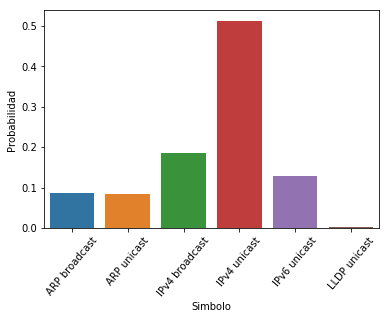
\includegraphics[width=\linewidth]{imagenes/despegar_barras_prob}
		\caption{Red corporativa - Probabilidad}
		\label{despe_barras_prob}
	\end{minipage}
	\begin{minipage}{0.49\textwidth}
		\centering
		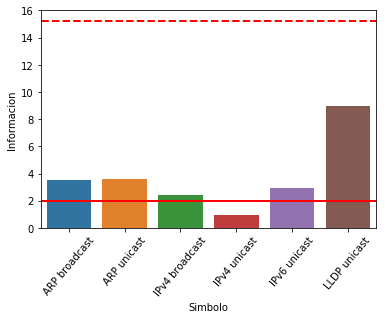
\includegraphics[width=\linewidth]{imagenes/despegar_barras_info}
		\caption{Red corporativa - Información}
		\label{despe_barras_info}
	\end{minipage}
\end{figure}

Sobre esta red observamos un trafico medianamente distribuido de los símbolos obtenidos. La mitad de ellos son \texttt{IPV4 UNICAST}, casi un 20 \% de \texttt{IPV4 BROADCAST} y entre 12\% y 8\% el resto. Puede verse una gran cantidad de informacion proveniente del símbolo \texttt{LLDP UNICAST}. Este protocolo es conocido cómo \textit{Link Layer Discovery Protocol}. La prescencia de este tipo de paquete se explica con que se usa como un componente en aplicaciones de administración y monitoreo de red, lo cual es común en redes corporativas. La baja frecuencia de este tipo de paquete repercute en que la información del símbolo sea muy alta.

Con el fin de realizar un análisis más exhaustivo, resulta útil estudiar los porcentajes relativos de aparición de los distintos símbolos de la fuente S1 para cada red.

\begin{figure}[H]
	\begin{minipage}{0.49\textwidth}
		\centering
		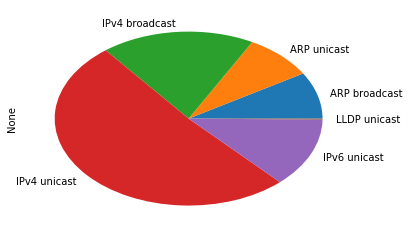
\includegraphics[width=\linewidth]{imagenes/despegar_torta_simbolos}
		\caption{Red corporativa - Símbolos}
		\label{despe_torta_simb}
	\end{minipage}
	\begin{minipage}{0.49\textwidth}
		\centering
		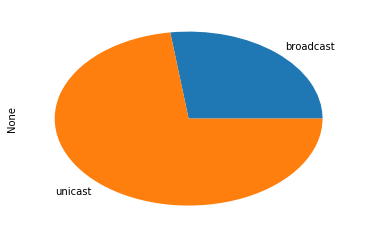
\includegraphics[width=\linewidth]{imagenes/despegar_torta_tipos}
		\caption{Red corporativa - Tipos}
		\label{despe_torta_tipos}
	\end{minipage}
\end{figure}

En este caso, existe una desproporción entre paquetes broadcast y unicast. Sin embargo, la proporción de paquetes broadcast y además la cantidad de paquetes ARP parece indicar que existe bastante interacción entre los nodos dentro de la red. Al ser una red con gran cantidad de hosts donde varios de ellos se comunican entre sí, estos necesitan mantenerse actualizados en cuanto a la información sobre la red. Es interesante observar la cantidad de paquetes tipo \texttt{IPV4 Broadcast}, este tipo de paquete es mayormente utilizado por protocolos de capas superiores, como NetBT, para tener más una mayor información sobre la red, ya que en un ambiente corporativo es muy necesario para detectar errores rápidamente.

\subsubsection{Red pública (McDonald's)}

\begin{figure}[H]
	\begin{minipage}{0.49\textwidth}
		\centering
		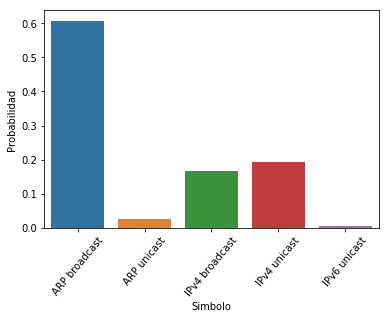
\includegraphics[width=\linewidth]{imagenes/mac_barras_prob}
		\caption{Red pública(McDonald's) - Probabilidad}
		\label{mac_barras_prob}		
	\end{minipage}
	\begin{minipage}{0.49\textwidth}
		\centering
		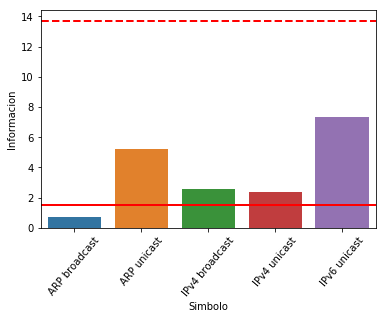
\includegraphics[width=\linewidth]{imagenes/mac_barras_info}
		\caption{Red pública(McDonald's) - Información}
		\label{mac_barras_info}		
	\end{minipage}
\end{figure}

La principal motivación para estudiar la red de McDonald's fue poder observar un medio con mucha entrada y salida de dispositivos, el hecho de que se tratara de una red inalámbrica permitió además contrastar las diferencias frente a la primer captura sobre una red cableada. Se nota la gran cantidad de paquetes \texttt{ARP BROADCAST}, son el 60\% de los capturados por lo que la información que proveen es escasa. Nuestra hipótesis es que la continua fluctuación de hosts en esta red provoca que se disparen muchos paquetes de control para mantener actualizado el estado de la misma. 

\begin{figure}[H]
	\begin{minipage}{0.49\textwidth}
		\centering
		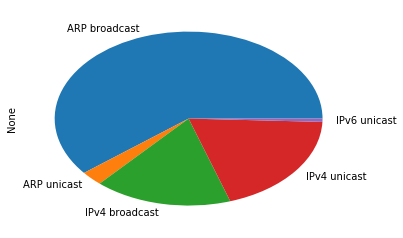
\includegraphics[width=\linewidth]{imagenes/mac_torta_simbolos}
		\caption{Red pública(McDonald's) - Símbolos}
		\label{mac_torta_simb}
	\end{minipage}
	\begin{minipage}{0.49\textwidth}
		\centering
		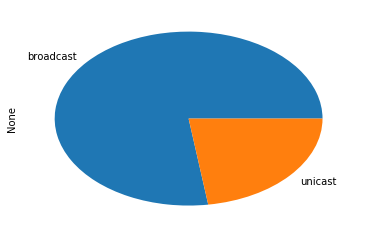
\includegraphics[width=\linewidth]{imagenes/mac_torta_tipos}
		\caption{Red pública(McDonald's) - Tipos}
		\label{mac_torta_tipos}
	\end{minipage}
\end{figure}

En la captura realizada sobre la red pública podemos ver que la cantidad de paquetes destinados al control de la red es considerablemente mayor con respecto a las red corporativa y la doméstica.

\subsubsection{Red doméstica}

\begin{figure}[H]
	\begin{minipage}{0.49\textwidth}
		\centering
		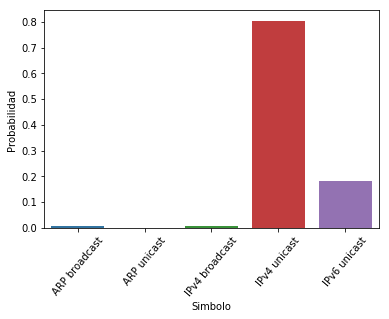
\includegraphics[width=\linewidth]{imagenes/manu_casa_barras_prob}
		\caption{Red doméstica - Probabilidad}
		\label{casa_barras_prob}
	\end{minipage}
	\begin{minipage}{0.49\textwidth}
		\centering
		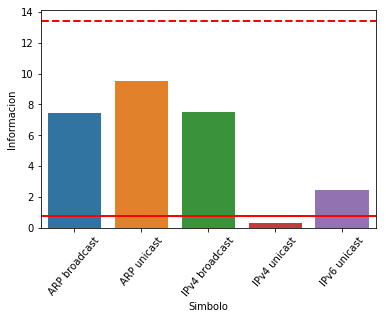
\includegraphics[width=\linewidth]{imagenes/manu_casa_barras_info}
		\caption{Red doméstica - Información}
		\label{casa_barras_info}
	\end{minipage}
\end{figure}

Para el grafico de la red doméstica podemos observar un predominancia en los paquetes \texttt{IPV4 UNICAST}, conformando mas de un 80\% de los paquetes que transitan por la red, seguido por un 18\% de paquetes \texttt{IPV6 UNICAST}. La entropía es de 0.797. Este número resulta mucho mas baja que las demás, y creemos que se debe justamente a que la gran mayoría de los paquetes es \texttt{UNICAST}, y esto provoca que el tráfico de la red sea fácil de predecir. La entropía es mucho menor en esta red que en las dos anteriores, lo cual indica una peor distribución en cuanto a los símbolos analizados. De la misma forma podemos observar que la red corporativa presenta una mejor distribución de los símbolos, lo cual se condice con su entropía, siendo esta la mayor de entre las tres redes.

\begin{figure}[H]
	\begin{minipage}{0.49\textwidth}
		\centering
		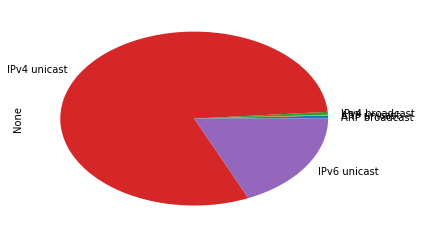
\includegraphics[width=\linewidth]{imagenes/manu_casa_torta_simbolos}
		\caption{Red doméstica - Símbolos}
		\label{casa_torta_simb}
	\end{minipage}
	\begin{minipage}{0.49\textwidth}
		\centering
		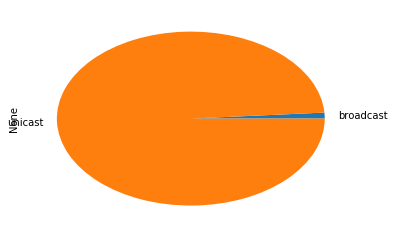
\includegraphics[width=\linewidth]{imagenes/manu_casa_torta_tipos}
		\caption{Red doméstica - Tipos}
		\label{casa_torta_tipos}
	\end{minipage}
\end{figure}

Como puede observarse en los gráficos, los resultados obtenidos para la fuente $S_1$ muestran que los paquetes de tipo broadcast son casi inexistentes. Este fenómeno se puede explicar, por el siguiente motivo: los paquetes de tipo broadcast suelen corresponder con protocolos de control, como ARP, y dado que las comunicaciones en general se dan exclusivamente entre el default gateway y los demás nodos, los protocolos de control no son requeridos.

\subsection{Modelo de fuente \texorpdfstring{$S_2$}{S2}}

Antes que nada, cabe destacar los cambios en la cantidad de símbolos con el modelo anterior. Este hace una distinción por cada host distinto dentro de las capturas, y al tener capturas en las que hay muchos dispositivos en juego, la cantidad de símbolos distintos aumenta linealmente con ellos.

\subsubsection{Red corporativa}

Dada la naturaleza de la red corporativa, es de esperarse que la cantidad de símbolos en $S_2$ sea elevada, ya que los mismos se distinguen por IP. Bajo nuestra categorización, encontramos un total de 239 símbolos.

\begin{figure}[H]
	\centering
	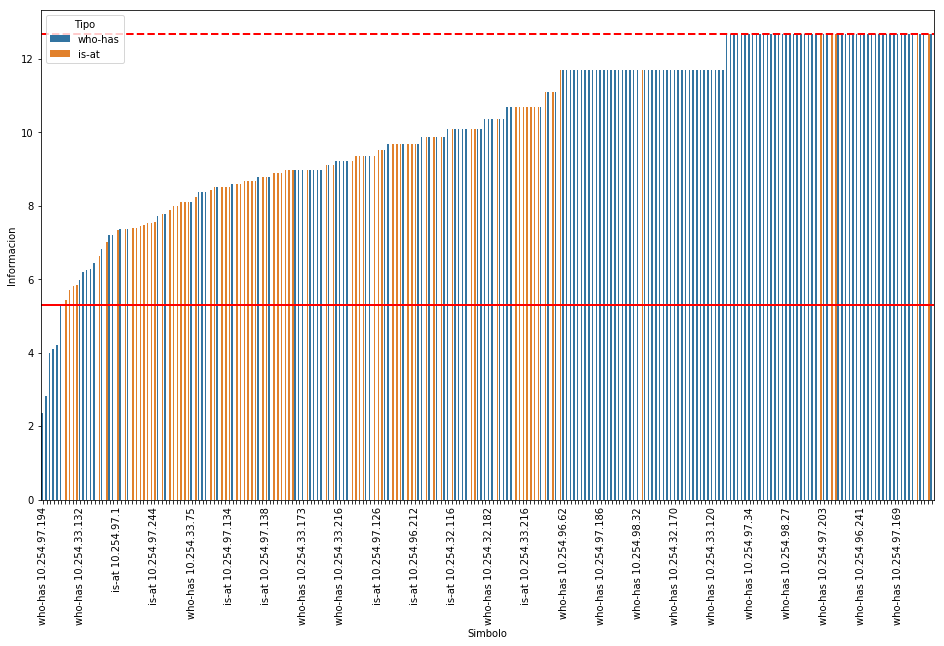
\includegraphics[width=\linewidth]{imagenes/despegar_barras_all}
	\caption{Red corporativa - Todos los símbolos}
\end{figure}

Pudimos observar que si bien hay más paquetes de tipo \texttt{WHO-HAS}, los paquete \texttt{IS-AT} no son pocos, casi el 25\% de los paquetes capturados, esto nos habla de una gran interacción entre los dispositivos pertenecientes a la red. En primera instancia, esperabamos encontrar una proporción cercana a 1:1, siendo que para cada pedido de \texttt{WHO-HAS} suele haber un nodo que lo responda. Nuestra hipótesis al respecto es que no tenemos acceso a todas las respuestas \texttt{IS-AT}, o también que esas redes no existen (pero esto es muy poco probable). Otra posible explicación es que la red está switcheada, lo cual justamente limita la cantidad de respuestas \texttt{IS-AT} que podemos ver porque limita la zona de colisión.

Un detalle que nos interesó en particular tiene que ver con los hosts que proveen menor informacion. Para ver esto, usamos un gráfico una pequeña porción de los hosts:

\begin{figure}[H]
	\centering
	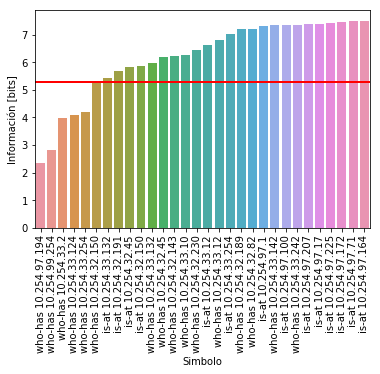
\includegraphics[width=.5\linewidth]{imagenes/despegar_hosts}
	\caption{Red corporativa}
\end{figure}

Puntualmente, hay 6 símbolos de tipo \texttt{WHO-HAS} por debajo de la entropía. Estos nodos distinguidos posiblemente sean las IPs referidas a gateways o a servidores que deben ser recurridos frecuentemente por distintos usuarios.

%TODO: Podemos decir que mas alla de que esos 6 dan poca informacion, hay otros que tambien dan poca inforamcion pero estan por arriba de la entropia por poco, podriamos decir que si bien son menos destacados que los 6 primeros son mucho mas frecuentes que el comun de los simbolos. (osea la entropía agarra a los mas distinguidos pero no a todos~~~~~)

\subsubsection{Red pública}

\begin{figure}[H]
	\centering
	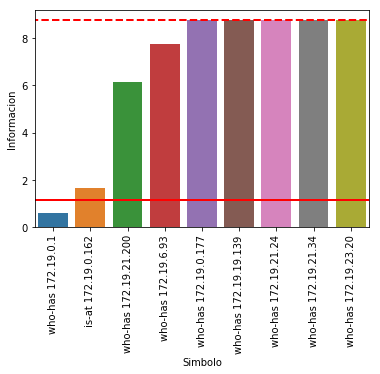
\includegraphics[width=.5\linewidth]{imagenes/mac_hosts}
	\caption{Red pública}
\end{figure}

Podemos observar que la cantidad de símbolos decreció abruptamente con respecto a la red anterior, y esto evidencia la diferencia de hosts que existe entre una red y otra. Era esperable que la cantidad de hosts sea mucho menor a la corporativa puesto que la primer red tiene muchos dispositivos destinados a la empresa mientras que la pública solo cuenta con algunos esporádicos clientes que deciden conectarse (por más que hayan muchos consumidores en el lugar, eso no significa que se conecten a la red).

Nótese que en el grafico la información del símbolo \texttt{WHO-HAS 172.19.0.1} se ubica por debajo de la entropía, es el que menos información aporta. Por ello deducimos que al ser un símbolo de \texttt{WHO-HAS}, 172.19.0.1 es el router, ya que es el más requerido. Podemos concluir esto último ya que cuanta menos información aporte mayor es su probabilidad de aparición.

% TODO: Hay que tneer en cuenta que para esta fuente filtramos los paquetes ARP de tipo gratuitous. Revisando los paquetes encontramos un protocolo de descubrimiento de dispositivos (SSDP), el cual despues de encontrar un paquete de tipo ssdp:discover, los dispositivos envian un paquete ARP gratuitous(is at destino y source iguales). Esto genera ruido e información que no necesitamos en el analisis.
 
\subsubsection{Red doméstica}

\begin{figure}[H]
	\centering
	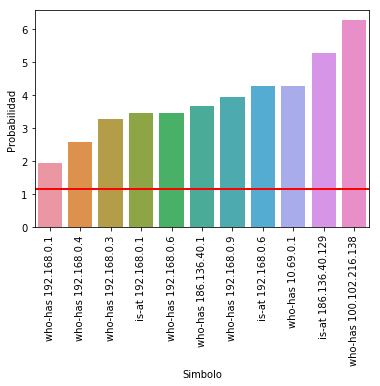
\includegraphics[width=.5\linewidth]{imagenes/manu_casa_hosts}
	\caption{Red doméstica}
\end{figure}


\section{Conclusión}

Un análisis interesante se origina al comparar las diferentes redes, las cuales tienen diferentes tecnologías subyacentes, y cómo esto afecta notoriamente a las fuentes de información estudiadas. Otro factor que afecta a las fuentes es el uso que se le da a la red, por ejemplo como el incremento de la actividad interna de la red aumenta la proporción de paquetes ARP dentro de la muestra, visto en la red empresarial. Sorprende la cantidad de paquetes que el usuario no percibe ya que son para el mantenimiento de la red.

Mediante el cálculo de la entropía podemos determinar que tan predecible es una red, a menor entropía es más fácil predecir.

Dejando de lado el análisis de la topología de la red por un momento, resulta interesante comparar la cantidad de información de los símbolos que aparecieron. En la figura 14 podemos notar que, efectivamente, hay símbolos que cargan mucha más información que otros. Si lo que buscamos es identificar nodos distinguidos, nos interesan los símbolos que cargan menor información, pues son los más frecuentes e indican actividad intensa (como puede ser la actividad correspondiente a un router).

Las zonas de colisión también juegan un factor importante en la recolección de datos ya que tendremos otra posibilidad de observar los paquetes que realmente viajan por la red. Este rasgo también se pudo evidenciar en los distintos análisis de las fuentes, al comparar los paquetes unicast contra los broadcast.

Nuestro modelos de análisis no es muy acertado, usamos fuentes de memoria nula cuando en realidad sabemos que, por ejemplo, captar la circulación de un paquete IS-AT es más probable si ya captamos un WHO-HAS. Sería interesante analizar cuales serian los resultados si tuviésemos en cuenta paquetes anteriores para determinar la probabilidad de uno nuevo.

Otras herramientas estadísticas como la moda de la muestra podrían ser útiles para encontrar símbolos distinguidos, sobre todo para la segunda fuente.



\end{document}
